\section{Grundlagen}
\subsection{Plasma}\label{sec:plasma}
Ein Gas, das teilweise oder vollständig ionisiert ist, wird als Plasma \cite{Plasmaphysik} bezeichnet. Bei der Ionisation dissoziieren die Gasteilchen in Elektronen und Ionen. Die Konzentration der beiden Ladungsarten ist ungefähr gleich groß. Deshalb ist ein Plasma nach außen hin neutral, obwohl es aus geladenen Teilchen besteht. Diese Eigenschaft wird als Quasineutralität bezeichnet. Damit verbunden ist die Eigenschaft, das ein Plasma elektromagnetische Felder abschirmen kann. 
Bevor ein ionisiertes Gas als Plasma bezeichnet werden kann, gibt es Bedienungen die erfüllt sein müssen.  Eine Bedingung ist, dass die Ausdehnung des ionisierten Gases deutlich größer ist als die Debye-Länge. Zusätzlich muss es eine hinreichend große Anzahl Teilchen geben, die sich innerhalb der Debye-Kugel befinden. Des weiteren muss die Zeit zwischen den Stößen zweier Gasteilchen viel größer als die Periodendauer der Plasmaoszillation sein. Bei der Plasmaoszillation handelt es sich um eine periodische Oszillation der Ladungsdichte. Die Ursache dafür ist, dass die Elektronen in den Potentialen der positiven Ionen schwingen. Die Frequenz der Oszillation ist die Plasmafrequenz
\begin{align}
\omega_{\mathrm{p}}=\sqrt{\frac{n_{\mathrm{e}}e^2}{\epsilon_0 m_{\mathrm{e}}}},
\end{align}
wobei $n_{\mathrm{e}}$ die Teilchenzahldichte der Elektronen, $m_{\mathrm{e}}$ die Elektronenmasse, $e$ die Elementarladung und $\epsilon_0$ die Dielektrizitätskonstante ist. Die Debye-Länge charakterisiert die Stärke der Abschirmung  eines Feldes durch ein Plasma. Die Debye-Länge $\lambda_{\mathrm{D}}$ ist die Länge, nach der das Feld auf das $1/e$ fache seines ursprünglichen Wertes abgefallen ist. Sie ist definiert als
\begin{align}
\lambda_{\mathrm{D}}=\sqrt{\frac{\epsilon_0 T}{e^2 n}},
\end{align}
wobei T die Temperatur und n die Teilchenzahldichte ist. Die Kugel mit der Debye-Länge als Radius wird als Debye-Kugel bezeichnet. In der Mitte der Kugel befindet sich ein geladenes Teilchen. Um dieses Teilchen befinden sich aufgrund der Coulomb-Wechselwirkung mehr entgegengesetzt geladenen Teilchen, als gleich geladene Teilchen. Folglich entsteht um das geladene Teilchen ein entgegengesetzt geladener Bereich. Dieser Bereich schirmt die Ladung nach außen hin ab.
Die Erzeugung eines Plasmas kann auf unterschiedliche Arten erfolgen. Eine erzwungene Ionisation von außen, zum Beispiel durch eine Glimmentladung, wird als unselbstständige Gasentladung bezeichnet. Der schematische Aufbau einer Glimmentladung und der Spannungsverlauf ist in der Abbildung \ref{fig:Glimmentladung} dargestellt.  Dabei wird an zwei Elektroden ein elektrisches Feld angelegt. Der Spannungsabfall zischen der Kathode und dem negativem Glimmlicht wird als Kathodenfall bezeichnet. Durch das elektrische Feld wird den Gasteilchen Energie zugeführt und diese dadurch ionisiert.  Die ionisierten Gasteilchen haben dadurch ausreichend Energie,  um  durch Stöße weitere Gasteilchen zu  Ionisieren. Dieser Vorgang wird als Stoßionisation bezeichnet. Eine Stoßionisation ist eine selbständige Gasentladung, da dieser Vorgang unabhängig von äußeren Einflüssen stattfinden kann. Die durchschnittliche Strecke die ein Teilchen zwischen zwei Stößen zurücklegen kann, wird als mittlere freie Weglänge bezeichnet. 
\begin{figure}[H]
\centering
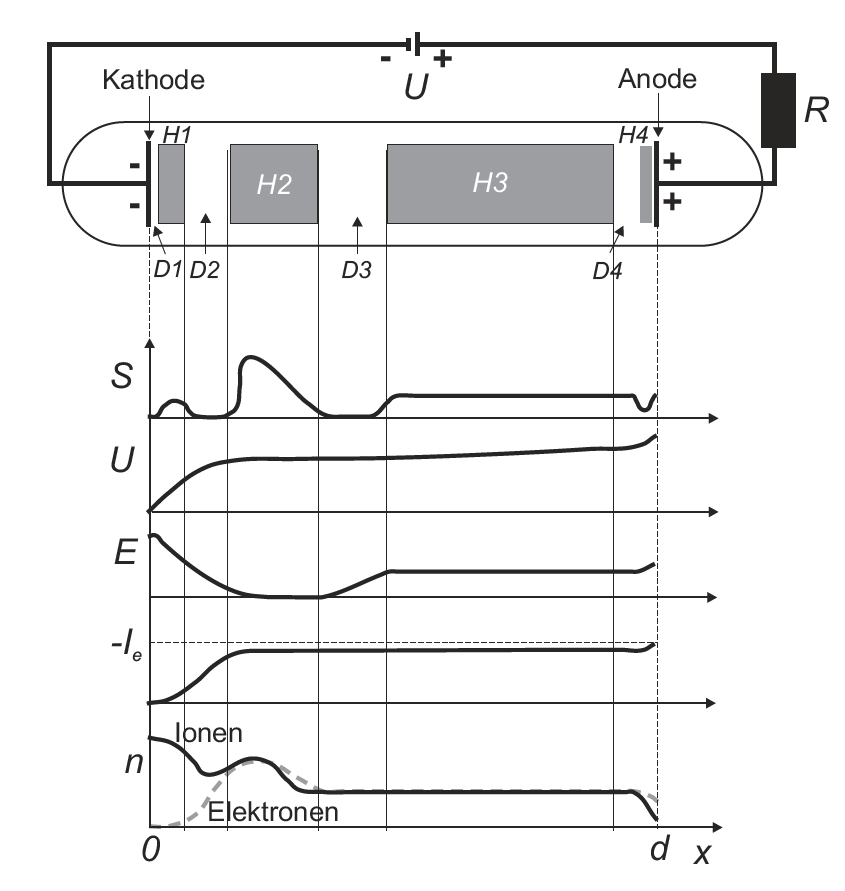
\includegraphics[scale=0.4]{Glimmentladung.png}
\caption{Schematischer Aufbau und Spannungsverlauf einer Glimmentladung.\cite{wiki:Glimmentladung}}
\label{fig:Glimmentladung}
\end{figure}
Bei den Ladungsträgern in einem Plasma handelt es sich um Elektronen und positiv geladenen Ionen. Das leichteste Ion wäre ein einzelnes Proton. Das Massenverhältnis zwischen den unterschiedlichen Ladungsträgern unterscheidet sich somit deutlich, da ein Proton ungefähr 1800 mal schwerer ist als ein Elektron. Dieser Unterschied ist für die Eigenschaften eines Plasmas von großer Bedeutung und kann auch für die Untersuchung eines Plasmas benutzt werden. Darauf wird im Kapitel \ref{sec:Langmuir_Sonde} detaillierter eingegangen. Bei einem Plasma kann häufig eine Leuchterscheinung beobachtet werden. Diese wird verursacht durch Strahlungsemission  der angeregten Atome. Bei sehr hohen und bei sehr tiefen Temperaturen gibt es dies nicht. Bei sehr tiefen Temperaturen sind keine Atome in einem angeregtem Zustand und somit kann auch kein Elektron auf einen Zustand niedriger Energie gelangen. Bei sehr hohen Temperaturen sind die Atome vollständig ionisiert und es gibt keine Elektronen mehr, die einen Übergang zwischen unterschiedlichen Energieniveaus machen könnten. Wie stark ein Plasma ionisiert ist, kann durch den  Ionisationsgrad angegeben werden. Der Ionisationsgrad ist null, im Fall eines neutralen Gases und eins, im Fall einer vollständigen Ionisierung. Der Abhängigkeit der Durchschlagspannung vom Gasdruck und der Schlagweite wird durch das Paschengesetz beschrieben. Unter der Durchschlagspannung versteht man die Spannung, ab der ein Isolator zu einem Plasma wird. 
\subsection{Langmuir-Sonde}\label{sec:Langmuir_Sonde}  
Eine Möglichkeit ein Plasma zu untersuchen ist die Verwendung von einer Langmuir-Sonde \cite{anleitung}. Damit können Eigenschaften des Plasmas wie Elektronendichte, Elektronentemperatur und Plasmapotential bestimmt werden. Die Schaltung zur Erzeugung eines Plasmas mit einer Glimmentladung und der Messung mit einer Langmuir-Sonde ist in der Abbildung \ref{fig:Schaltung_Sonde} dargestellt. 
\begin{figure}[H]
\centering
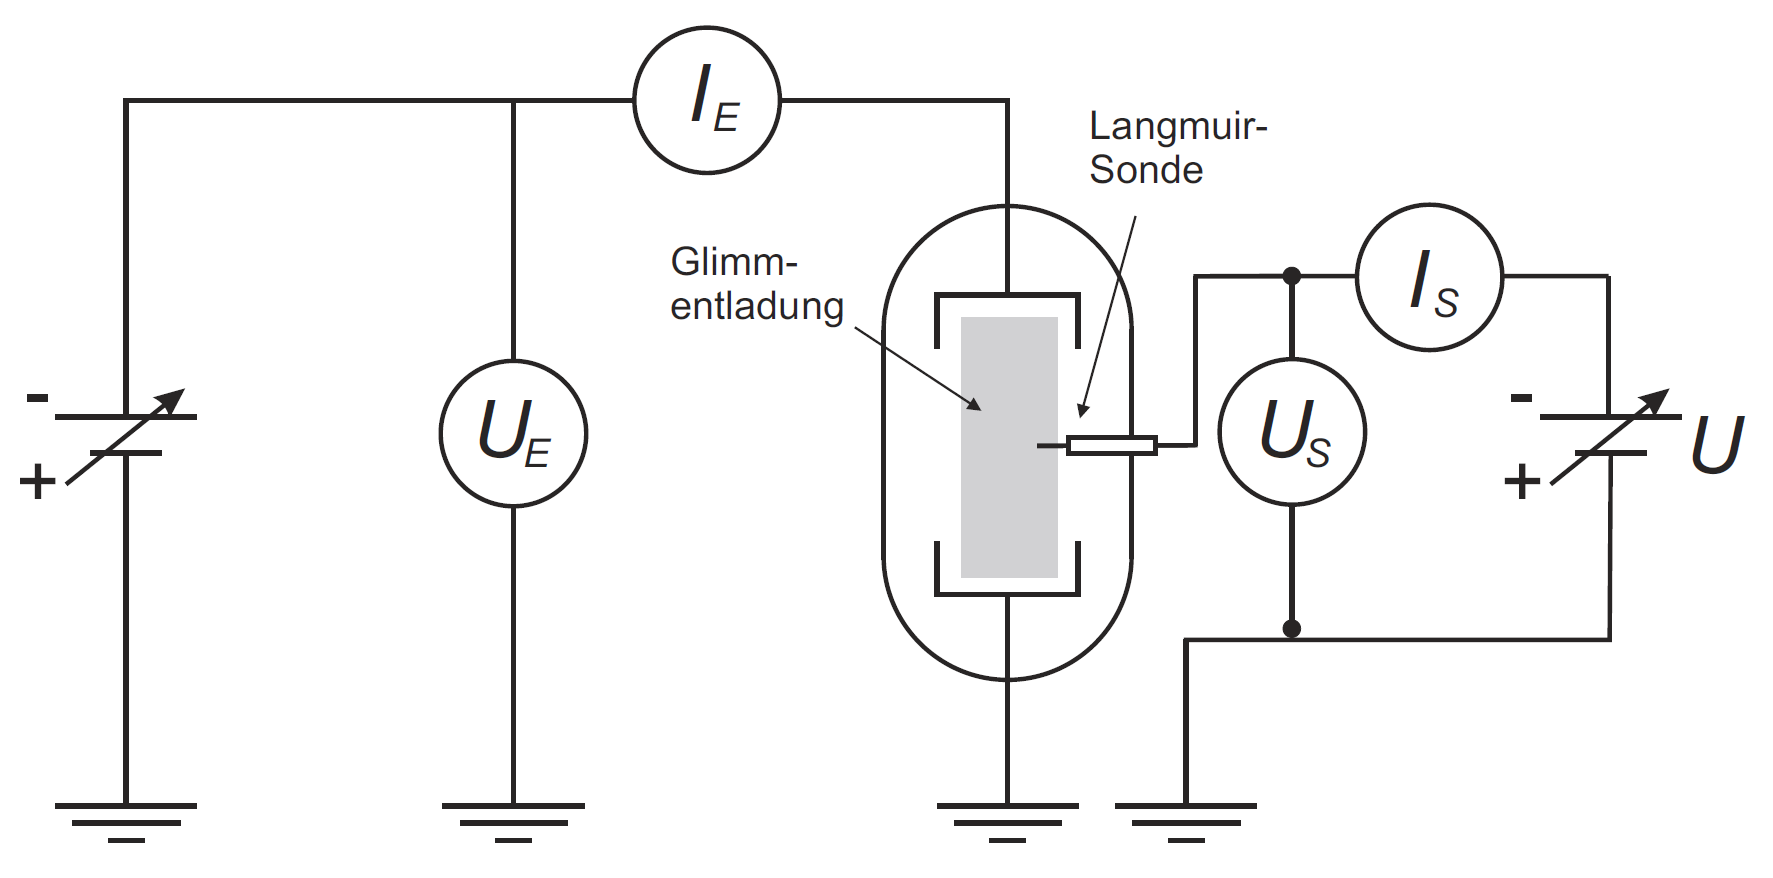
\includegraphics[scale=0.4]{Schaltung_Sonde.PNG}
\caption{Schaltung zur Erzeugung eines Plasmas mit einer Glimmentladung und der Messung mit einer Langmuir-Sonde. \cite{anleitung}}
\label{fig:Schaltung_Sonde}
\end{figure}
Die Spitze einer Langmuir-Sonde besteht aus einer Elektrode, die wiederum meistens aus einem dünnem Wolfram-Draht besteht. Die Sonde ist außer an der Spitze isoliert. Das Potential der Sonde unterscheidet sich von dem Potential des Plasmas. Dies kann durch das im Kapitel \ref{sec:plasma} erläuterte Massenverhältnis zwischen positiven und negativen Ladungsträger erklärt werden. Aufgrund ihrer geringeren Masse haben Elektronen eine höhere Mobilität. Bei gleicher Elektronen- und Ionentemperatur sind die Elektronen somit schneller als die Ionen. Dadurch treffen Elektronen häufiger auf die Sonde als die Ionen. Die Sonde lädt sich somit negativ auf. Durch das negative Aufladen der Sonde entsteht eine elektrostatische Kraft, die Elektronen abstößt und  Ionen anzieht. Im Gleichgewichtszustand wird die höhere Mobilität durch die elektrostatische Abstoßung kompensiert. Das heißt, die Elektronen- und Ionenströme sind gleich groß. Das Potential der Sonde das sich im Gleichgewichtsfall einstellt, wird als Floatingpotential $\Phi_{\mathrm{fl}}$ bezeichnet. In der Kennlinie \ref{fig:Kennlinie_Sonde} entspricht dies dem  Nulldurchgang.  Um den Rest der Kennlinie zu messen, muss eine Spannung an die Sonde angelegt werden. Wird die Sonde negativ aufgeladen, werden Elektronen abgestoßen und Ionen angezogen. Bei einer ausreichend starken negativen Aufladung, sind alle Ionen aus de Umgebung der Sonde angezogen worden. Die Stromstärke steigt nun bei noch stärkerer negativen Spannung  nicht mehr an und wird als Ionensättigungstrom bezeichnet. Dies ist der Bereich im Diagramm \ref{fig:Kennlinie_Sonde}, bei dem ein konstanter positiver Strom gemessen werden kann. Der Sättigungsstrom kann mit
\begin{align}
 I_{\mathrm{i},\mathrm{sat}}=0.61enS \sqrt{\frac{T_\mathrm{e}}{m_{\mathrm{i}}}},
\end{align} 
 wobei $T_{\mathrm{e}}$ die Elektronentemperatur, $S$ die effektive Sondenoberfläche und $m_{\mathrm{i}}$ die Ionenmasse ist, berechnet werden. Analog zum Ionensättigungsstrom kann auch ein Elektronensättigungsstrom gemessen werden. Dazu muss die Sonde ausreichen positiv geladen sein, damit alle Elektronen aus der Umgebung der Sonde von dieser angezogen worden sind. Im Idealfall einer unendlich ausgedehnten, ebenen Sonde wird der Elektronensättigungsstrom konstant. In dem Diagramm der Kennlinie ist dies der Bereich, mit dem konstantem negativem Strom. Berechnet werden kann der Elektronensättigungsstrom mit
\begin{align}
I_{\mathrm{e},\mathrm{sat}}=-enS \sqrt{\frac{T_{\mathrm{e}}}{2\pi m_{\mathrm{e}}}}.
\label{eq:Ionensaettigungsstrom}
\end{align}
Der Idealfall lässt sich experimentell nicht realisieren, das heißt das die Stromstärke nicht konstant bleibt, wenn die Spannung steigt. An der Stelle, an der die reale Kennlinie größer wird als der Elektronensättigungsstrom, gibt es einen Knick in der Kennlinie. Die Stelle, an der der Knick ist, wird als Plasmapotential bezeichnet. Das heißt, der Elektronenlaufbereich endet am Plasmapotential. Der Verlauf der Kennlinie für größere Stromstärken als der Elektronensättigungsstrom, ist von der Geometrie der Sonde anhängig. Der Bereich zwischen den Sättigungsströmen wird Elektronenlaufbereich genannt. In diesem Bereich können nur die Elektronen die Sonde erreichen, die  ausreichend thermische Energie haben. Die Elektronenstrom im Elektronenlaufbereich ist gegeben durch
\begin{align}
I_{\mathrm{e}}=I_{\mathrm{e},\mathrm{sat}}\ \mathrm{exp} \left( -\frac{e(\Phi_{\mathrm{p}}-U)}{T_{\mathrm{e}}} \right),
\label{eq:Elektronenlaufbereich}
\end{align}
wobei $\Phi_{\mathrm{p}}$ das Plasmapotential und $U$ die angelegte Spannung an der Sonde ist. Der gesamte Strom im Elektronenlaufbereich ist die Summe aus Elektronenstrom und Ionenstrom
\begin{align}
I=I_{\mathrm{e}} +  I_{\mathrm{i},\mathrm{sat}}=  I_{\mathrm{e},\mathrm{sat}}\ \mathrm{exp} \left( -\frac{e(\Phi_{\mathrm{p}}-U)}{T_{\mathrm{e}}} \right) + I_{\mathrm{i},\mathrm{sat}}.
\end{align}
Dies lässt sich umformen in
\begin{align}
\mathrm{ln}(I_{\mathrm{i},\mathrm{sat}} -I) = \mathrm{ln}(I_{\mathrm{e},\mathrm{sat}}) - \frac{e(\Phi_{\mathrm{p}}-U)}{T_{\mathrm{e}}}.
\end{align}
Aus der Kennlinie kann der Ionensättigungsstrom abgelesen werden. Durch die Korrektur des Gesamtstromes durch den Ionensättigungsstrom, kann man im einem halb-logarithmischem Diagramm aus dem Offset die  Dichte und aus der Steigung die Elektronentemperatur bestimmen. 
\begin{figure}[H]
\centering
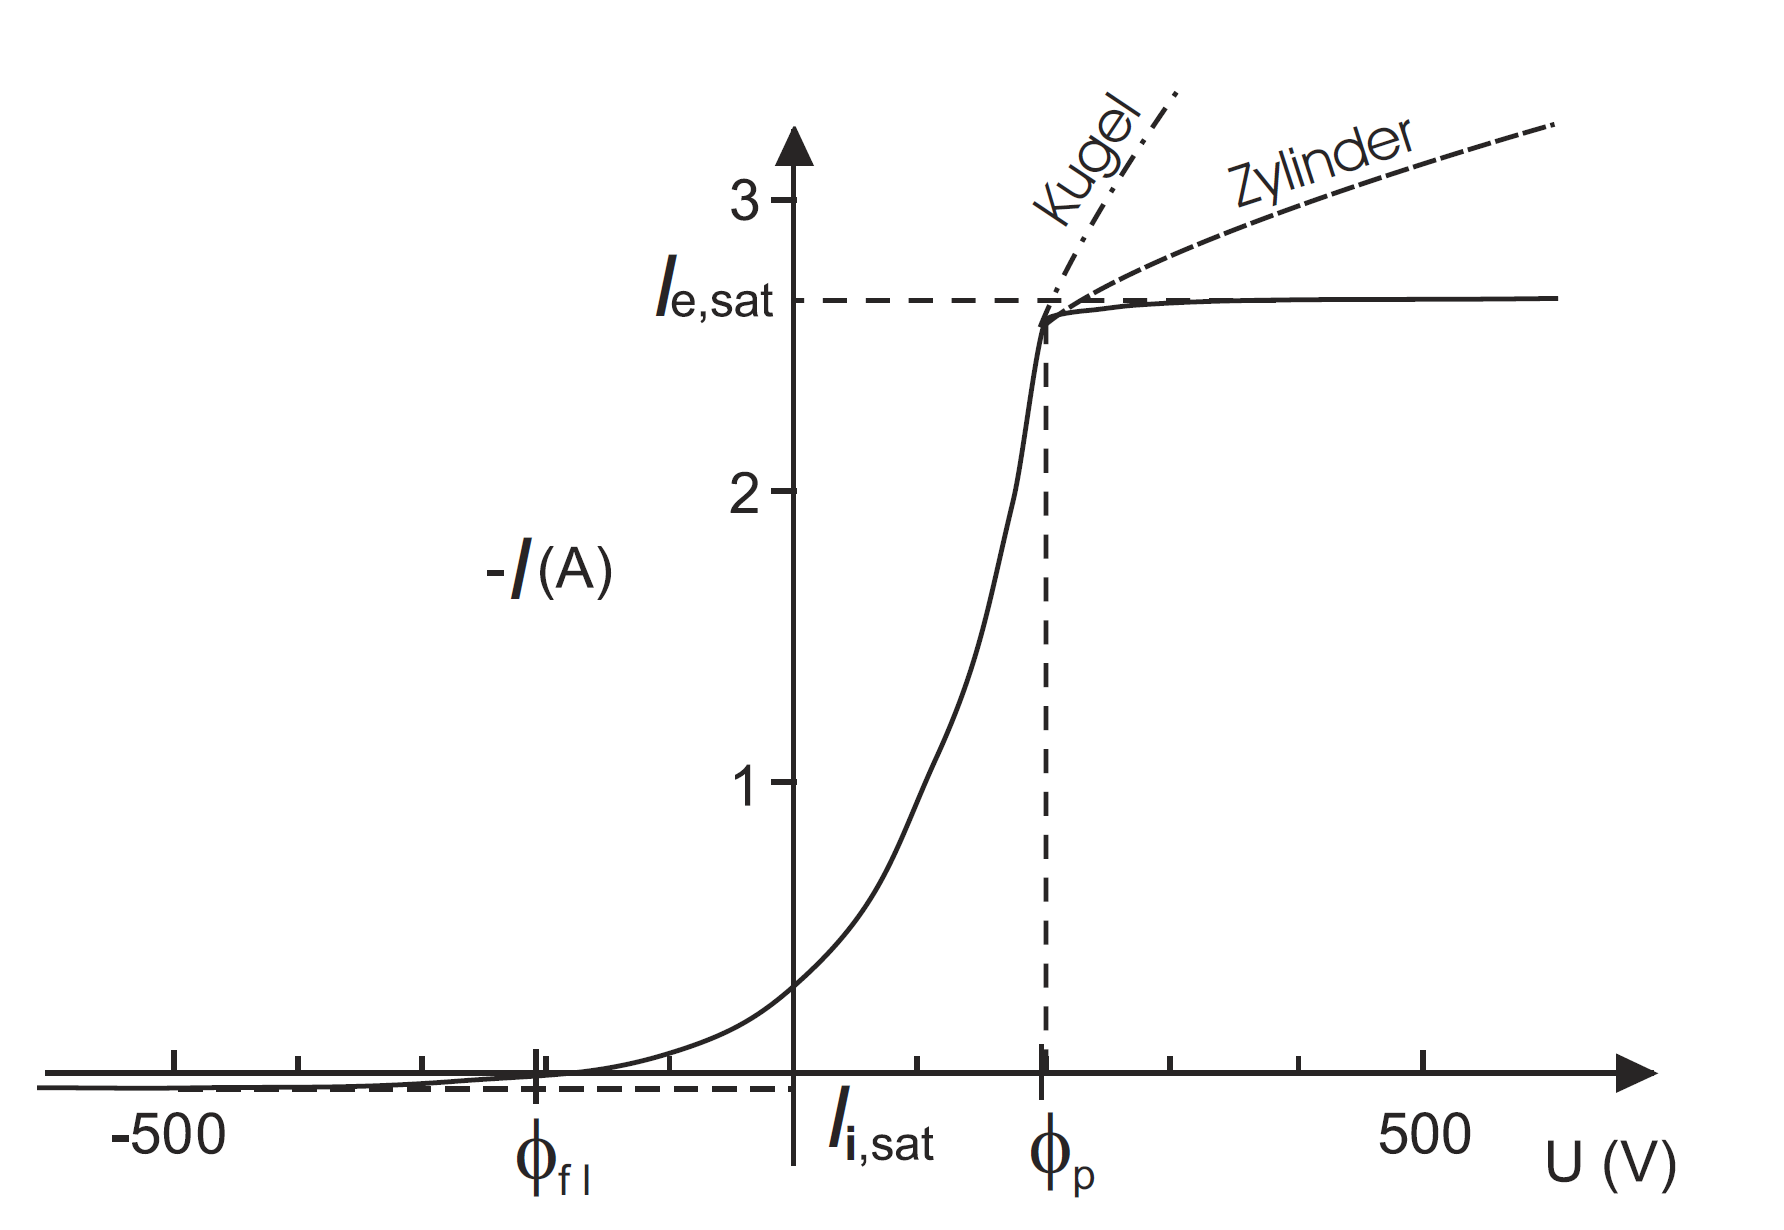
\includegraphics[scale=0.4]{Kennlinie_Sonde.PNG}
\caption{Kennlinie einer Langmuir-Sonde. \cite{anleitung}}
\label{fig:Kennlinie_Sonde}
\end{figure}
\subsection{Doppel-Sonde}
Für die Messung mit einer einzelnen Langmuir-Sonde wird ein Referenzpotential benötigt, welches jedoch nicht immer möglich ist (zum Beispiel auf einem Satelliten). In so einem Fall, kann eine Doppel-Sonde \cite{anleitung} verwendet werden, da dafür kein Referenzpotential notwendig ist. Die Schaltung für eine Doppelsonde ist in der Abbildung \ref{fig:Schaltung_Doppel_Sonde} dargestellt. In der Abbildung sieht man, das der Strom dabei von der einen Sonde durch das Plasma zur anderen Sonde fließt. 

\begin{figure}[H]
\centering
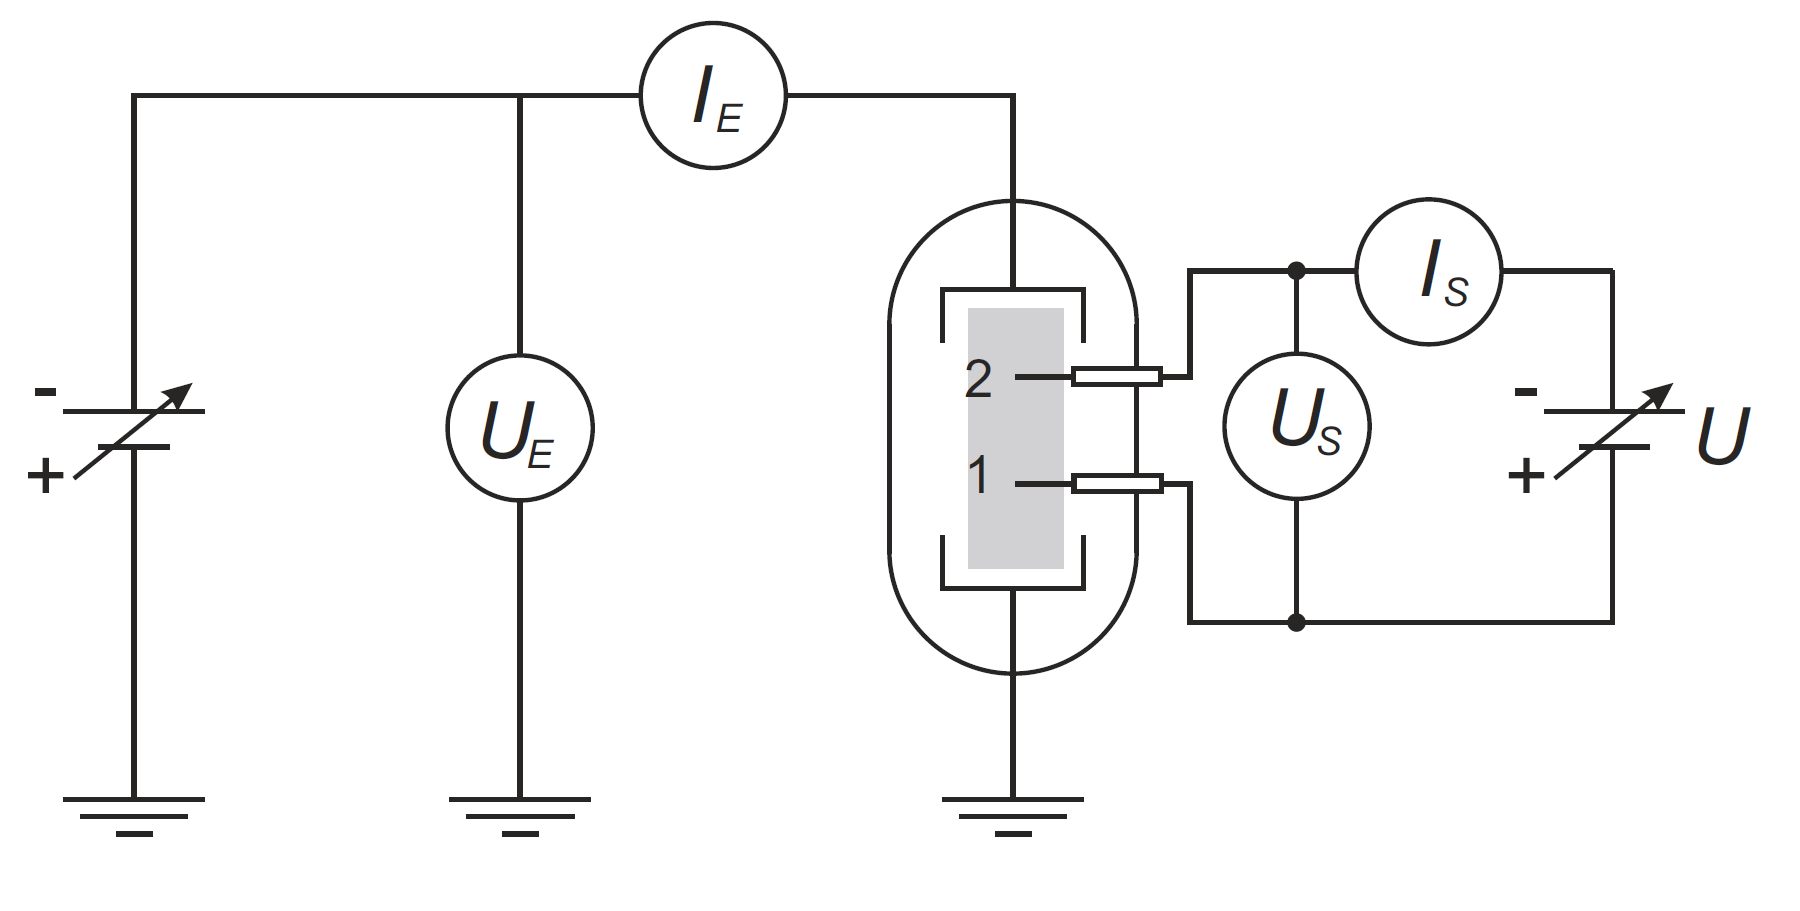
\includegraphics[scale=0.4]{Schaltung_Doppel_Sonde.PNG}
\caption{Schaltung zur Erzeugung eines Plasmas mit einer Glimmentladung und der Messung mit einer Doppel-Sonde. \cite{anleitung}}
\label{fig:Schaltung_Doppel_Sonde}
\end{figure}
Für die Messung wird wie bei der Langmuir-Sonde die Spannung variiert und der Strom gemessen.  Die Kennlinie einer Doppelsonde ist in der Abbildung \ref{fig:Kennlinie_Doppel_Sonde} dargestellt. Wird an die Doppelsonde keine Spannung angelegt, fließt auch kein Strom. Das bedeutet der Nulldurchgang der Kennlinie ist im Ursprung.  In diesem Fall ist das System im Gleichgewicht und analog zur Langmuir-Sonde wird das Potential der beiden Sonden als Floatingpotential bezeichnet. Bei sehr großen Spannungen, sowohl negativ als auch positiv, geht der Strom in den Ionensättigungsbereich über. Der Verlauf der Kennlinie im Sättigungsbereich hängt von der Geometrie der beiden Sonden ab. Bei identischen Sonden, ist die Kennlinie punktsymmetrisch zum Ursprung. Zwischen den Bereichen mit der Elektronensättigung ist der Elektronenlaufbereich. 
\begin{figure}[H]
\centering
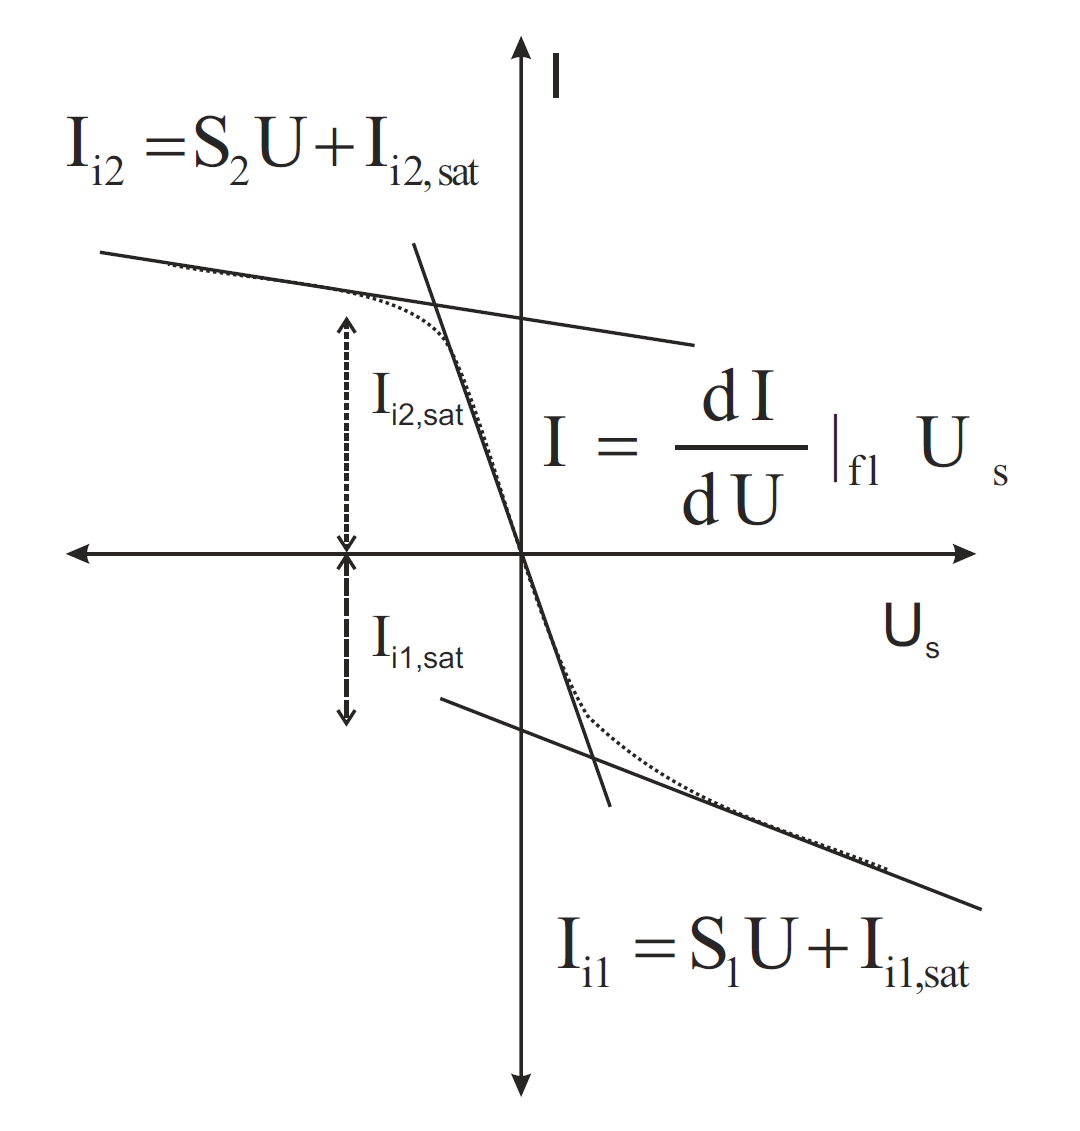
\includegraphics[scale=0.4]{Kennlinie_Doppel_Sonde.PNG}
\caption{Kennlinie einer Doppel-Sonde. \cite{anleitung}}
\label{fig:Kennlinie_Doppel_Sonde}
\end{figure}
Der gesamte Sondenstrom ist die Summe der Beiträge von den Elektronen und den Ionen gemäß
\begin{align}
I_{\mathrm{S}}=I_{\mathrm{e}1} -I_{\mathrm{i}1} = I_{\mathrm{i}2} -I_{\mathrm{e}2}.
\label{eq:Gesamter_strom}
\end{align} 
Für den Elektronenlaufbereich gilt mit \eqref{eq:Elektronenlaufbereich}
\begin{align}
I_{\mathrm{e}1} &=I_{\mathrm{e}1,\mathrm{sat}}\ \mathrm{exp} \left( -\frac{e(\Phi_{\mathrm{p}}-U_1)}{T_{\mathrm{e}}} \right) \label{eq:ELektronenlaufbereich_Doppel_sonde1} \\
I_{\mathrm{e}2} &=I_{\mathrm{e}2,\mathrm{sat}}\ \mathrm{exp} \left( -\frac{e(\Phi_{\mathrm{p}}-U_2)}{T_{\mathrm{e}}} \right). 
\label{eq:ELektronenlaufbereich_Doppel_sonde2}
\end{align}
Mit den Gleichung \eqref{eq:Gesamter_strom} und  \eqref{eq:Ionensaettigungsstrom} und der Spannung $U=U_1-U_2$ lässt sich der Ausdruck
\begin{align}
\frac{I_{\mathrm{S}} + I_{\mathrm{i}1}}{ I_{\mathrm{i}2} - I_{\mathrm{S}}}= \frac{I_{\mathrm{e}1}}{I_{\mathrm{e}2}}= \frac{S_1}{S_2} \mathrm{exp} \left( \frac{e U_{\mathrm{S}}}{T_{\mathrm{e}}} \right)
\end{align}
herleiten. Aus der Annahme das $I_{\mathrm{i}1}$ und $I_{\mathrm{e}2}$ unabhängig von $U_{\mathrm{S}}$ sind, folgt aus de Gleichung \eqref{eq:Gesamter_strom}
\begin{align}
\frac{\mathrm{d} I_{\mathrm{S}}}{\mathrm{d} U_{\mathrm{S}}}= \frac{\mathrm{d} I_{\mathrm{e}1}}{\mathrm{d} U_{\mathrm{S}}}= -\frac{\mathrm{d} I_{\mathrm{e}2}}{\mathrm{d} U_{\mathrm{S}}}.
\label{eq.Ableitung_strom}
\end{align}
Durch einsetzen der Gleichungen \eqref{eq:ELektronenlaufbereich_Doppel_sonde1} und \eqref{eq:ELektronenlaufbereich_Doppel_sonde2} in die Gleichung \eqref{eq.Ableitung_strom} folgt
\begin{align}
I_{\mathrm{e}1,\mathrm{sat}}\ \mathrm{exp} \left( \frac{e U_1}{T_{\mathrm{e}}} \right) \frac{\mathrm{d} U_1}{\mathrm{d} U_{\mathrm{S}}} + I_{\mathrm{e}2,\mathrm{sat}}\ \mathrm{exp} \left( \frac{e U_2}{T_{\mathrm{e}}} \right)  \left( \frac{\mathrm{d} U_1}{\mathrm{d} U_{\mathrm{S}}} -1 \right) =0.
\end{align}
Bei einer angelegten Spannung von $U=0$ V gilt $U_1=U_2=U_{\mathrm{fl}}$, daraus folgt
\begin{align}
\left. \frac{\mathrm{d} U_1}{\mathrm{d} U_{\mathrm{S}}}\right\vert_{U_{\mathrm{S}}=0}= \frac{I_{\mathrm{e}2,\mathrm{sat}}}{I_{\mathrm{e}1,\mathrm{sat}}+I_{\mathrm{e}2,\mathrm{sat}}}=\frac{I_{\mathrm{i}2,\mathrm{sat}}}{I_{\mathrm{i}1,\mathrm{sat}}+I_{\mathrm{i}2,\mathrm{sat}}}.
\label{eq:Ableitung_2}
\end{align}  
Aus den Gleichungen \eqref{eq.Ableitung_strom} und \eqref{eq:Ableitung_2} kann die Ableitung der Sondenkennlinie bei $U_{\mathrm{S}}=0$ 
\begin{align}
\left. \frac{\mathrm{d} I_{\mathrm{S}}}{\mathrm{d} U_{\mathrm{S}}}\right\vert_{U_{\mathrm{S}}=0} = \frac{e}{T_{\mathrm{e}}}  \frac{I_{\mathrm{i}2,\mathrm{sat}}}{I_{\mathrm{i}1,\mathrm{sat}}+I_{\mathrm{i}2,\mathrm{sat}}}  I_{\mathrm{e}1,\mathrm{sat}}\ \mathrm{exp} \left( \frac{e(\Phi_{\mathrm{p}}-\Phi_{\mathrm{fl}})}{T_{\mathrm{e}}}\right)
\end{align}
bestimmt werden. Gilt für die angelegte Spannung $U_1=U_{\mathrm{fl}}$, folgt damit
\begin{align}
I_{\mathrm{e}1,\mathrm{sat}} =I_{\mathrm{e}1,\mathrm{sat}}\ \mathrm{exp} \left( -\frac{e(\Phi_{\mathrm{p}}-U_1)}{T_{\mathrm{e}}} \right).
\end{align}
Daraus ergibt sich
\begin{align}
\left. \frac{\mathrm{d} I_{\mathrm{S}}}{\mathrm{d} U_{\mathrm{S}}}\right\vert_{U_{\mathrm{S}}=0} = \frac{e}{T_{\mathrm{e}}}\frac{I_{\mathrm{i}1,\mathrm{sat}} I_{\mathrm{i}2,\mathrm{sat}} }{I_{\mathrm{i}1,\mathrm{sat}}+I_{\mathrm{i}2,\mathrm{sat}}}.
\end{align}
Durch fitten von zwei Geraden an die beiden Ionensättigungsbereiche und kann durch eine Interpolation der Ionensättigungsstrom bestimmt werden. Aus den Schnittpunkten der Geraden mit der Achse für die Stromstärke, können die Ionensättigungsströme ermittelt werden. Daraus kann die Plasmadichte bestimmt werden.  Aus der Steigung der Kennlinie im Elektronenlaufbereich kann die Elektronentemperatur bestimmt werden.  
\subsection{RC-Glied}
RC-Glieder sind Schaltungen, die aus einem Widerstand und einem Kondensator bestehen.  Aus RC-Gliedern lassen sich zum Beispiel Hoch- und Tiefpassfilter realisieren. Bei einem Tiefpassfilter, wie in der Abbildung \ref{fig:Hochpass_Teifpass} dargestellt, ist der Kondensator parallel am Signalausgang geschaltet, während bei einem Hochpassfilter die Position des Widerstandes mit dem des Kondensators vertauscht ist.   
\begin{figure}[H]
\centering
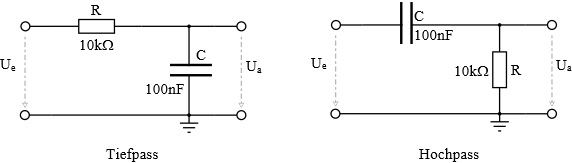
\includegraphics[scale=0.6]{Hochpass_Tiefpass.jpg}
\caption{Schaltung eines Hochpass- und eines Teifpassfilters. \cite{Hochpass_Tiefpass}}
\label{fig:Hochpass_Teifpass}
\end{figure}
